
  % 1. a identificação do projeto;
  % 2. a introdução;
  % 3. as atividades desenvolvidas;
  % 4. os resultados obtidos; e
  % 5. as considerações finais.

%% abtex2-modelo-relatorio-tecnico.tex, v-1.9.6 laurocesar
%% Copyright 2012-2016 by abnTeX2 group at http://www.abntex.net.br/ 
%%
%% This work may be distributed and/or modified under the
%% conditions of the LaTeX Project Public License, either version 1.3
%% of this license or (at your option) any later version.
%% The latest version of this license is in
%%   http://www.latex-project.org/lppl.txt
%% and version 1.3 or later is part of all distributions of LaTeX
%% version 2005/12/01 or later.
%%
%% This work has the LPPL maintenance status `maintained'.
%% 
%% The Current Maintainer of this work is the abnTeX2 team, led
%% by Lauro César Araujo. Further information are available on 
%% http://www.abntex.net.br/
%%
%% This work consists of the files abntex2-modelo-relatorio-tecnico.tex,
%% abntex2-modelo-include-comandos and abntex2-modelo-references.bib
%%

% ------------------------------------------------------------------------
% ------------------------------------------------------------------------
% abnTeX2: Modelo de Relatório Técnico/Acadêmico em conformidade com 
% ABNT NBR 10719:2015 Informação e documentação - Relatório técnico e/ou
% científico - Apresentação
% ------------------------------------------------------------------------ 
% ------------------------------------------------------------------------

\documentclass[
  % -- opções da classe memoir --
  12pt,       % tamanho da fonte
  % openright,      % capítulos começam em pág ímpar (insere página vazia caso preciso)
  % twoside,      % para impressão em recto e verso. Oposto a oneside
  oneside,
  a4paper,      % tamanho do papel. 
  % -- opções da classe abntex2 --
  %chapter=TITLE,   % títulos de capítulos convertidos em letras maiúsculas
  %section=TITLE,   % títulos de seções convertidos em letras maiúsculas
  %subsection=TITLE,  % títulos de subseções convertidos em letras maiúsculas
  %subsubsection=TITLE,% títulos de subsubseções convertidos em letras maiúsculas
  % -- opções do pacote babel --
  english,      % idioma adicional para hifenização
  french,       % idioma adicional para hifenização
  spanish,      % idioma adicional para hifenização
  brazil,       % o último idioma é o principal do documento
  ]{abntex2}


% ---
% PACOTES
% ---

% ---
% Pacotes fundamentais 
% ---
\usepackage{lmodern}      % Usa a fonte Latin Modern
\usepackage[T1]{fontenc}    % Selecao de codigos de fonte.
\usepackage[utf8]{inputenc}   % Codificacao do documento (conversão automática dos acentos)
\usepackage{indentfirst}    % Indenta o primeiro parágrafo de cada seção.
\usepackage{color}        % Controle das cores
\usepackage{graphicx}     % Inclusão de gráficos
\usepackage{microtype}      % para melhorias de justificação
% ---

% ---
% Pacotes adicionais, usados no anexo do modelo de folha de identificação
% ---
\usepackage{multicol}
\usepackage{multirow}
% ---
  
% ---
% Pacotes adicionais, usados apenas no âmbito do Modelo Canônico do abnteX2
% ---
\usepackage{lipsum}       % para geração de dummy text
% ---

% ---
% Pacotes de citações
% ---
\usepackage[brazilian,hyperpageref]{backref}   % Paginas com as citações na bibl
\usepackage[alf]{abntex2cite} % Citações padrão ABNT

% --- 
% CONFIGURAÇÕES DE PACOTES
% --- 

% ---
% Configurações do pacote backref
% Usado sem a opção hyperpageref de backref
\renewcommand{\backrefpagesname}{Citado na(s) página(s):~}
% Texto padrão antes do número das páginas
\renewcommand{\backref}{}
% Define os textos da citação
\renewcommand*{\backrefalt}[4]{
  \ifcase #1 %
    Nenhuma citação no texto.%
  \or
    Citado na página #2.%
  \else
    Citado #1 vezes nas páginas #2.%
  \fi}%
% ---

% ---
% Informações de dados para CAPA e FOLHA DE ROSTO
% ---
\titulo{Filtro de Partículas Aplicado à\\Localização de Robôs Móveis\\no Domínio da RoboCup Humanoide}
\autor{Aislan Cesar de Almeida}
\local{São Bernardo do Campo - SP}
\data{Outubro 2017}
\instituicao{%
  Centro Universitário da
  \par
  Fundação Educacional Inaciana Pe. Sabóia de Medeiros - FEI
  \par
  Programa de Pós-Graduação em Engenharia Elétrica
  \par
  Departamento de Inteligência Artificial Aplicada à Automação.}
\tipotrabalho{Relatório de Atividades}
% O preambulo deve conter o tipo do trabalho, o objetivo, 
% o nome da instituição e a área de concentração 
\preambulo{Relatório das atividades desenvolvidas durante o período em que o autor foi bolsista do Conselho Nacional de Desenvolvimento Científico e Tecnológico com o objetivo de obter o título de Mestre de Ciência.}
% ---

% ---
% Configurações de aparência do PDF final

% alterando o aspecto da cor azul
\definecolor{blue}{RGB}{41,5,195}
\definecolor{black}{RGB}{0,0,0}

% informações do PDF
\makeatletter
\hypersetup{
      %pagebackref=true,
    pdftitle={\@title}, 
    pdfauthor={\@author},
      pdfsubject={\imprimirpreambulo},
      pdfcreator={LaTeX with abnTeX2},
    pdfkeywords={abnt}{latex}{abntex}{abntex2}{relatório técnico}, 
    colorlinks=true,          % false: boxed links; true: colored links
      linkcolor=black,           % color of internal links
      citecolor=black,           % color of links to bibliography
      filecolor=magenta,          % color of file links
    urlcolor=blue,
    bookmarksdepth=4
}
\makeatother
% --- 

% --- 
% Espaçamentos entre linhas e parágrafos 
% --- 

% O tamanho do parágrafo é dado por:
\setlength{\parindent}{1.3cm}

% Controle do espaçamento entre um parágrafo e outro:
\setlength{\parskip}{0.2cm}  % tente também \onelineskip

% ---
% compila o indice
% ---
\makeindex
% ---

% ----
% Início do documento
% ----
\begin{document}

% Seleciona o idioma do documento (conforme pacotes do babel)
%\selectlanguage{english}
\selectlanguage{brazil}

% Retira espaço extra obsoleto entre as frases.
\frenchspacing 

% ----------------------------------------------------------
% ELEMENTOS PRÉ-TEXTUAIS
% ----------------------------------------------------------
% \pretextual

% ---
% Capa
% ---
\imprimircapa
% ---

% ---
% Folha de rosto
% (o * indica que haverá a ficha bibliográfica)
% ---
\imprimirfolhaderosto*
% ---

% ---
% Anverso da folha de rosto:
% ---

% {
% \ABNTEXchapterfont

% \vspace*{\fill}

% Conforme a ABNT NBR 10719:2015, seção 4.2.1.1.1, o anverso da folha de rosto
% deve conter:

% \begin{alineas}
%   \item nome do órgão ou entidade responsável que solicitou ou gerou o
%    relatório; 
%   \item título do projeto, programa ou plano que o relatório está relacionado;
%   \item título do relatório;
%   \item subtítulo, se houver, deve ser precedido de dois pontos, evidenciando a
%    sua subordinação ao título. O relatório em vários volumes deve ter um título
%    geral. Além deste, cada volume pode ter um título específico; 
%   \item número do volume, se houver mais de um, deve constar em cada folha de
%    rosto a especificação do respectivo volume, em algarismo arábico; 
%   \item código de identificação, se houver, recomenda-se que seja formado
%    pela sigla da instituição, indicação da categoria do relatório, data,
%    indicação do assunto e número sequencial do relatório na série; 
%   \item classificação de segurança. Todos os órgãos, privados ou públicos, que
%    desenvolvam pesquisa de interesse nacional de conteúdo sigiloso, devem
%     informar a classificação adequada, conforme a legislação em vigor; 
%   \item nome do autor ou autor-entidade. O título e a qualificação ou a função
%    do autor podem ser incluídos, pois servem para indicar sua autoridade no
%    assunto. Caso a instituição que solicitou o relatório seja a mesma que o
%    gerou, suprime-se o nome da instituição no campo de autoria; 
%   \item local (cidade) da instituição responsável e/ou solicitante; NOTA: No
%    caso de cidades homônimas, recomenda-se o acréscimo da sigla da unidade da
%    federação.
%   \item ano de publicação, de acordo com o calendário universal (gregoriano),
%   deve ser apresentado em algarismos arábicos.
% \end{alineas}

% \vspace*{\fill}
% }

% ---
% Agradecimentos
% ---
% \begin{agradecimentos}
% O agradecimento principal é direcionado a Youssef Cherem, autor do
% \nameref{formulado-identificacao} (\autopageref{formulado-identificacao}).

% Os agradecimentos especiais são direcionados ao Centro de Pesquisa em
% Arquitetura da Informação\footnote{\url{http://www.cpai.unb.br/}} da Universidade de
% Brasília (CPAI), ao grupo de usuários
% \emph{latex-br}\footnote{\url{http://groups.google.com/group/latex-br}} e aos
% novos voluntários do grupo
% \emph{\abnTeX}\footnote{\url{http://groups.google.com/group/abntex2} e
% \url{http://www.abntex.net.br/}}~que contribuíram e que ainda
% contribuirão para a evolução do abn\TeX.

% \end{agradecimentos}
% ---

% ---
% RESUMO
% ---

% resumo na língua vernácula (obrigatório)
\setlength{\absparsep}{10pt} % ajusta o espaçamento dos parágrafos do resumo
\begin{resumo}
  Este relatório apresenta as atividades desempenhadas pelo autor durante a vigência da bolsa auxílio do programa de mestrado, concedida pelo Conselho Nacional de Desenvolvimento Científico e Tecnológico (CNPq).
  Esse relatório se faz necessário por determinação do próprio CNPq, para concluir a vigência do contrato de bolsa.
  A principal atividade realizada neste período foi a obtenção do título de mestre pelo autor.

  O objetivo do mestrado foi implementar um sistema de localização em robôs humanoides autônomos.
  Para que robôs humanoides possam jogar futebol competitivamente de maneira autônoma é necessário que os robôs conheçam suas posições no campo, essa informação é essencial para o desenvolvimento de estratégias.
  A posição pode ser estimada a partir do conhecimento de como o robô se move pelo domínio e por observações feitas pelo próprio robô.
  Mas isso não é uma tarefa trivial.
  Os movimentos executados pelos robôs são imprecisos, além de problemas não modeláveis que surgem por problemas da parte física do robô.
  As observações feitas pelo robô são ruidosas, o que impedem que informações precisas de direção e distância sejam obtidas, pois seus poucos sensores estão em constante movimento devido ao balanço necessário para manter o robô em movimento.

  É comum encontrar trabalhos acadêmicos sobre localização de robôs autônomos para diversos domínios, mas são poucos os trabalhos que lidam com um domínio tão restrito quanto o deste trabalho.
  Além disso, os trabalhos sobre este domínio apresentam algoritmos e resultados que não são reprodutíveis, devido às diferenças de \textit{hardware} e \textit{software} dos robôs utilizados.
  Assim, este trabalho implementa um sistema de localização, baseado no algoritmo de localização de Monte-Carlo, para que robôs humanoides autônomos sejam capazes de estimar suas posições no domínio.
  
  O sistema implementado apresenta um método para estimar o quanto o robô se move ao longo do tempo e métodos diferentes para calcular quanto cada partícula representa a posição do robô real, além de métodos para se recuperar de erros de estimativa, para alterar a quantidade de partículas conforme o necessário e para estimar qual a melhor observação que o robô poderá fazer em instantes futuros.
  Foram realizados experimentos simulados e em robôs reais que validam os métodos implementados e mostram que os métodos propostos são eficientes para resolver o problema de localização.
  Por fim, trabalhos futuros incluem verificar o funcionamento do sistema em situação de jogo, além da expansão do sistema para um domínio genérico para observar o funcionamento dos métodos propostos e compará-las à outros métodos do estado da arte.

  \noindent
  \textbf{Palavras-chaves}: filtro de partículas. localização de monte-carlo. localização de robô. robô humanoide. futebol de robôs. relatório de atividades.
\end{resumo}
% ---

% ---
% inserir lista de ilustrações
% ---
\pdfbookmark[0]{\listfigurename}{lof}
\listoffigures*
\cleardoublepage
% ---

% ---
% inserir lista de tabelas
% ---
% \pdfbookmark[0]{\listtablename}{lot}
% \listoftables*
% \cleardoublepage
% ---

% ---
% inserir lista de abreviaturas e siglas
% ---
\begin{siglas}  
  \item[BRAHUR] \textit{Brazilian Humanoid Robot Workshop}, \textit{Workshop} de Robôs Humanoides do Brasil
  \item[CNPq] Conselho Nacional de Desenvolvimento Científico e Tecnológico
  \item[FEI] Centro Universitário da Fundação Educacional Inaciana Pe. Sabóia de Medeiros
  \item[LARC] \textit{Latin American Robotics Competition}, ou Competição Latino-Americana de Robótica
  \item[LARS] \textit{Latin American Robotics Symposium}, Simpósio Latino-Americano de Robótica
  \item[MCL] Localização de Monte-Carlo
  \item[OBR] Olimpíada Brasileira de Robótica
\end{siglas}
% ---

% ---
% inserir lista de símbolos
% ---
% \begin{simbolos}
%   \item[$ \Gamma $] Letra grega Gama
%   \item[$ \Lambda $] Lambda
%   \item[$ \zeta $] Letra grega minúscula zeta
%   \item[$ \in $] Pertence
% \end{simbolos}
% ---

% ---
% inserir o sumario
% ---
\pdfbookmark[0]{\contentsname}{toc}
\tableofcontents*
\cleardoublepage
% ---


% ----------------------------------------------------------
% ELEMENTOS TEXTUAIS
% ----------------------------------------------------------
\textual

\chapter{Introdução}

O processo de localização é definido neste trabalho como o ato do robô de estimar sua própria posição no domínio.
É possível inferir a posição do robô no campo a partir de observações de características discrepantes do mundo e conhecendo as ações realizadas pelo robô.
Por sua vez, a posição é um conjunto de informações que indicam onde um robô se encontra no mundo, a qual deve ser capaz de descrever, sem ambiguidade, qualquer ponto do mundo no qual o robô está inserido.

\citeonline{art:RoboCup} explica que o domínio da \textit{RoboCup Soccer Humanoid League}, exige que os robôs possuam características humanas.
Desta forma, eles devem se mover como pessoas, e seus sensores são limitados a sensores que imitem os sentidos humanos.
Além disso, os robôs precisam ser totalmente autônomos, ou seja, tomar decisões e coordenar estratégias sem auxílios externos.
Para que as decisões e estratégias sejam eficientes, os robôs precisam conhecer suas posições no campo.
A figura~\ref{fig:robocup} apresentam os robôs que participaram da \textit{RoboCup Soccer Humanoid League}, que foi realizada em Nagoya, Japão, em Julho de 2017.

\begin{figure}[b]
  \centering
  \caption{Foto dos robôs que participaram na RoboCup de 2017 em Nagoya.}\label{fig:robocup}
    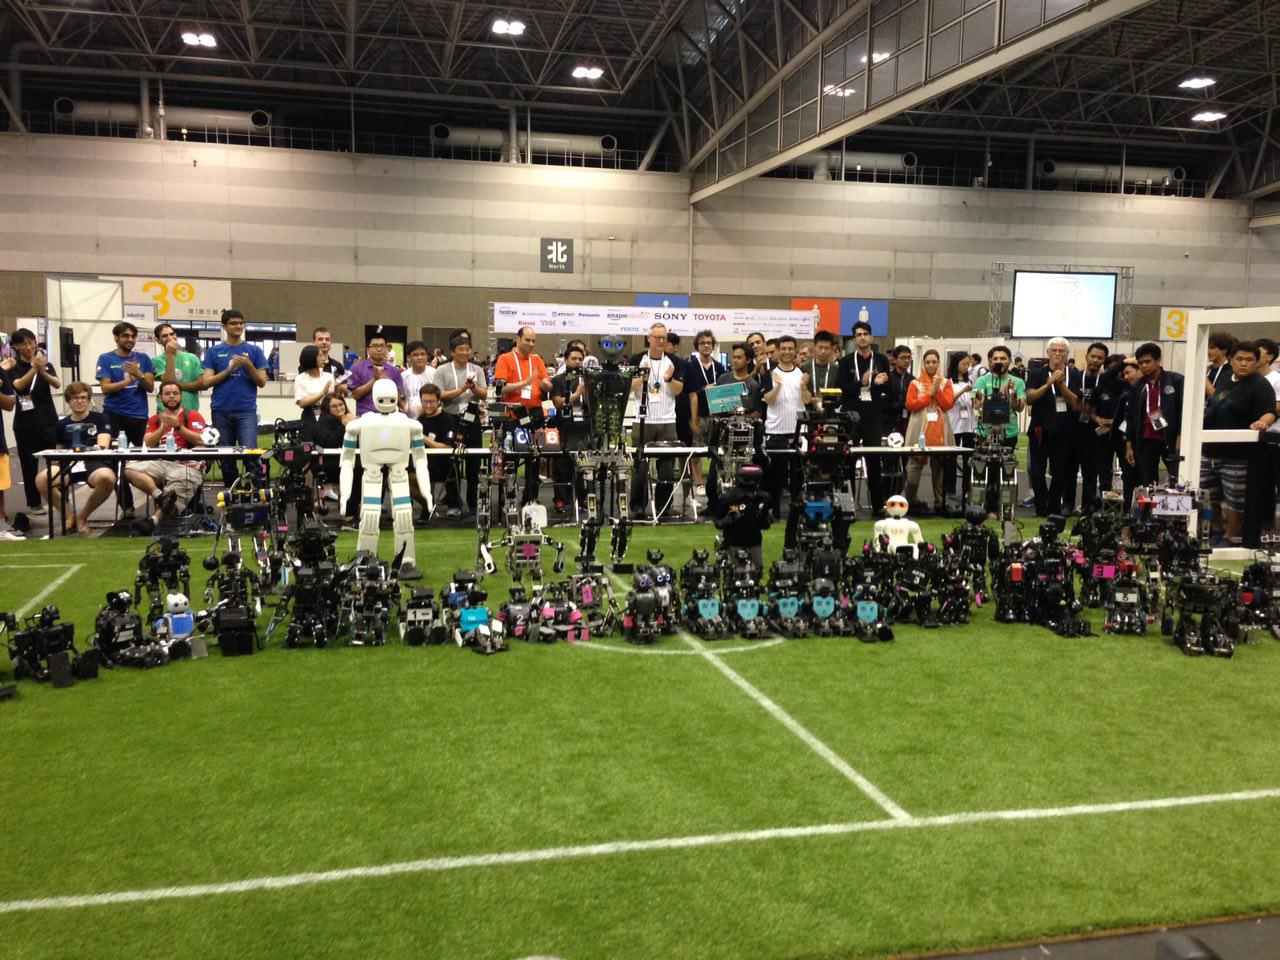
\includegraphics[width=\textwidth, trim={0 5cm 0 5cm}, clip]{fig/robocup2017}
\end{figure}

Conforme o robô se move ele deve manter um ritmo de balanço, de maneira que ele consiga manter o equilíbrio enquanto anda.
Esse balanço faz com que a câmera esteja em constante movimento, gerando observações ruidosas.
A figura~\ref{fig:visioncamera} apresenta uma imagem obtida pela câmera do robô em movimento.
Ainda que alguma característica seja identificada, é praticamente impossível determinar qual a distância exata entre o robô e a característica observada.
Além disso, as características podem ser ocluídas em situações diversas, ou ainda, o robô pode não conseguir identificar a característica por ela estar muito distante.

\begin{figure}[t]
  \centering
  \caption{Imagem vista pela câmera do robô em movimento.}\label{fig:visioncamera}
    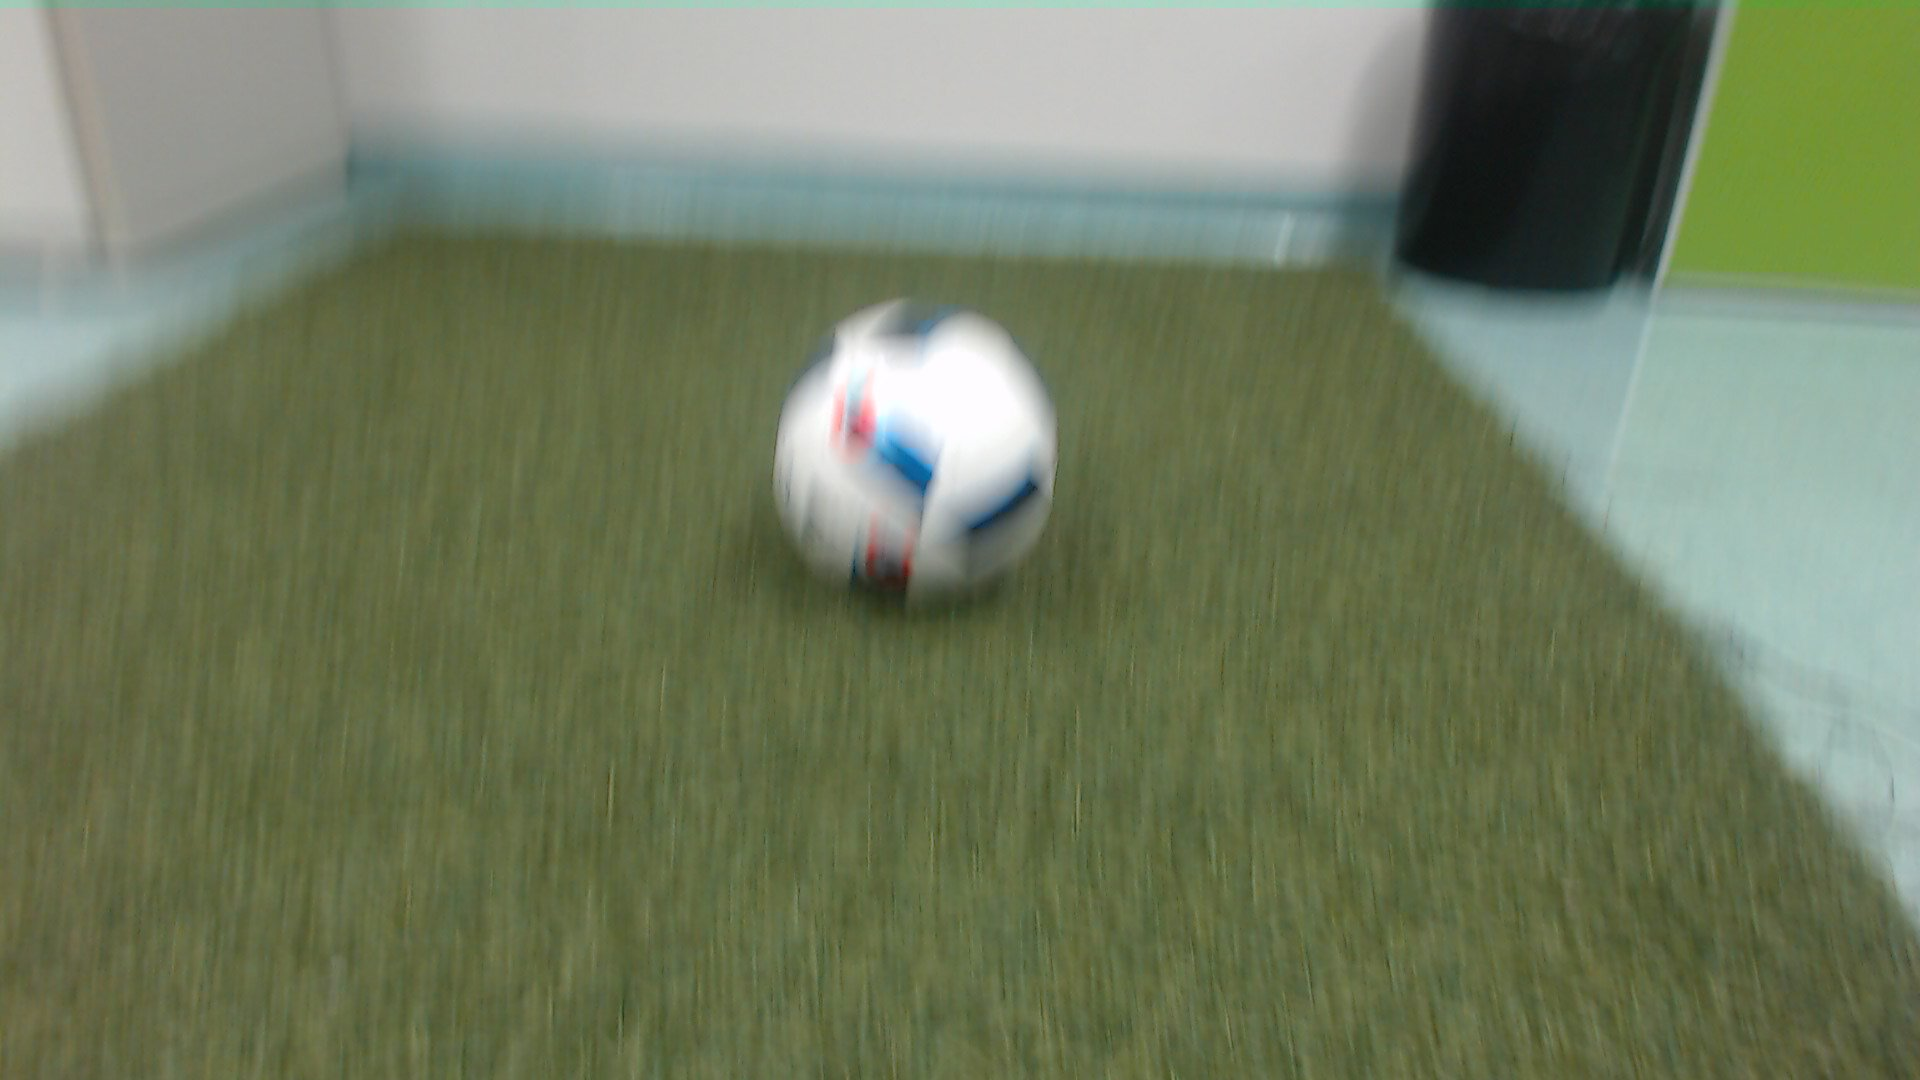
\includegraphics[width=0.8\textwidth, height=0.45\textwidth]{fig/foto}
\end{figure}

Além da câmera, os robôs podem usar sensores inerciais e retroalimentação do posicionamento dos servo-motores como informação para reconstituir a trajetória feita pelo robô, no entanto esses sensores acumulam erros ao longo do tempo.
Além disso, o movimento dos robôs é errático, pois eles estão sujeitos à quedas, folgas nas juntas, escorregamento e imprecisão no posicionamento dos servo-motores.
Por fim, cada robô tem um comportamento único devido às suas características físicas.

Não é uma tarefa trivial fazer com que um robô autônomo se localize em um ambiente real.
A incerteza gerada pelos movimentos imprecisos do robô e pelos sensores ruidosos impossibilitam determinar a posição exata do robô.
No entanto, é possível inferir quais posições tem maior probabilidade de representar a localização atual do robô no mundo.
Segundo \citeonline{russell2010artificial} isso é feito através da inferência em redes bayesianas dinâmicas.

Assim, o objetivo deste trabalho é apresentar um sistema de localização baseado no método probabilístico de inferência aproximada em redes Bayesianas dinâmicas conhecido como Localização de Monte-Carlo (MCL), proposto por \citeonline{dellaert1999monte} e \citeonline{fox1999monte}.
O sistema é capaz de estimar a posição do robô no mundo e se recuperar de erros de estimativa, alterando a quantidade de partículas de maneira que o equilíbrio entre a qualidade da estimativa e o tempo de execução seja mantida, além de apresentar um método que determina qual observação deve ser feita para melhorar a estimativa da posição.

Ainda que seja comum encontrar métodos baseados no MCL aplicados à diversos domínios uma nova implementação se faz necessária, de maneira que todas as peculiaridades do domínio deste trabalho sejam consideradas.
O método apresentado neste trabalho considera as falhas de movimento dos robôs, os ruídos contidos nas observações feitas pelos robôs e as limitações de hardware e software para apresentar um sistema de localização funcional para robôs humanoides autônomos.

O MCL modela os erros de movimento e observação, além de resolver os três principais problemas de localização: a localização global, o rastreamento de posição e o problema do sequestro.
A localização global é a situação na qual o robô desconhece sua posição inicial e deve estimar sua posição conforme ele se move e observa o ambiente.
O rastreamento de posição é a situação na qual a posição do robô é atualizada conforme ele se move.
Por fim, o problema do sequestro é quando o robô precisa recuperar-se de uma estimativa errada de posição.
A posição estimada estará errada quando o robô é movido de uma posição conhecida para uma desconhecida, ou quando o robô sofre algum erro de movimento não modelado pelo modelo de movimento.

Os robôs utilizados para experimentos neste trabalho possuem limitações de \textit{hardware} e \textit{software}, que podem deixar o sistema de localização excessivamente lento.
Um bom sistema de localização deve ser capaz de retornar a posição estimada do robô em tempo real, que no caso do domínio deste trabalho será considerado um período de $1$ segundo, no máximo.
Além disso, o sistema de localização é executado em paralelo com vários outros sistemas essenciais para o funcionamento do robô, de maneira que se o sistema de localização for computacionalmente custoso isso pode prejudicar o funcionamento do robô como um todo.

Para implementar a localização de robôs humanoides autônomos este trabalho propõe a implementação de um algoritmo de localização baseado no MCL.
O trabalho propõe a implementação de um modelo de movimento baseado em velocidade para robôs omnidirecionais, três modelos de observação e um método de reamostragem de partículas que trabalha em tempo linear em função das quantidades de partículas.
Além de apresentar três contribuições para o estado da arte dos métodos de localização:
a dispersão de partículas de baixa representatividade, com o objetivo de recuperar o filtro de erros de estimativa;
o método que adapta a quantidade de partículas à distribuição probabilística, para economizar recursos computacionais;
e um método que estima qual observação deve prover a melhor informação para o sistema de localização.

%--------------------------------------------------------------------------------------------------

\chapter{Atividades Desenvolvidas}

A principal atividade desenvolvida foi a obtenção do título de mestre, cujas etapas serão descritas na seção~\ref{sec:projeto}.
Em paralelo com isso foram desenvolvidas outras atividades que envolveram participações voluntárias em eventos e cursos oferecidos pela FEI, que serão descritas na seção~\ref{sec:extra}.

\section{Obtenção do Título de Mestre}\label{sec:projeto}

A FEI exige, para concluir o mestrado, a obtenção de seis créditos em disciplinas.
Esses créditos foram obtidos no primeiro ano, onde as disciplinas cursadas foram:
%
\begin{enumerate}
  \item \textbf{Inteligência Computacional} que teve o objetivo de introduzir os principais algoritmos de otimização e aprendizado de padrões, no caso redes neurais, algoritmos genéticos e lógica fuzzy, na qual o conceito obtido foi B;

  \item \textbf{Algoritmos Computacionais} que apresentou diversos algoritmos de ordenação, busca e introduziu os paradigmas da computação, na qual o conceito obtido foi A;

  \item \textbf{Engenharia de Software em Experimentos Científicos} que apresentou os conceitos relacionados à engenharia de software, aplicados em experimentos científicos, com o objetivo de ensinar métodos para documentar e apresentar experimentos com relevância científica, o conceito obtido nesta matéria foi A;

  \item \textbf{Fundamentos de Inteligência Artificial} que apresenta fundamentos da lógica proposicional, o funcionamento dos métodos de busca e vários outros conceitos pertinentes aos métodos de inteligência artificial, o conceito obtido nesta matéria foi A;

  \item \textbf{Inteligência Artificial Probabilística} que apresenta os conceitos de probabilidades, teoria de jogos, métodos probabilísticos de inferência e raciocínio, na qual o conceito obtido foi B;

  \item \textbf{Programação Científica} na qual os alunos devem implementar diversos algoritmos e testá-los de maneira científica, gerando relatórios sobre cada método, na qual o conceito obtido foi A.
\end{enumerate}

Após a conclusão das matérias, iniciou-se o processo de escrita da qualificação, que culminou na apresentação realizada em 07 de Abril de 2017.
A qualificação compreendeu toda a teoria e a proposta que seria desenvolvida.
A banca concordou que o trabalho era relevante para a área e que valia um mestrado, qualificando o autor à receber o título.
Para tanto, foram desenvolvidas as seguintes teorias concernentes ao processo de localização:
%
\begin{enumerate}
  \item um modelo de movimento que considera apenas qual o movimento executado pelo robô para alterar as posições das partículas no mundo;

  \item modelos de observação que seriam utilizados para ponderar os pesos das partículas;

  \item e um método para reamostragem das partículas em função de seus pesos, que tem tempo de execução linearmente proporcional à quantidade de partículas.
\end{enumerate}

Em seguida iniciou-se o processo de desenvolvimento e implementação das teorias.
Que além da implementação dos métodos previamente apresentados, também foram desenvolvidas:
%
\begin{enumerate}
  \item a implementação de um método de recuperação de erros de estimativa, caracterizado pelo problema do sequestro;

  \item a implementação de um método que varia a quantidade de partículas de acordo com a necessidade do filtro de partículas;

  \item e a implementação de um método que estima de qual observação deve se obter a melhor informação para o processo de localização.
\end{enumerate}
%
Em seguida, os métodos foram implementados em simulação e em robôs reais, nos quais foram feitos experimentos para avaliar as técnicas.
Finalmente, o processo foi finalizado com a escrita e defesa da dissertação, que ocorreu no dia 18 de Setembro de 2017.
Após analisar o trabalho e testar o autor sobre a qualidade e conhecimento concernentes à dissertação apresentada, a banca julgou que o autor era digno de receber o título de mestre.
Agora o autor deve revisar alguns trechos da dissertação e corrigi-los para entregar a versão final à biblioteca da FEI.

\section{Atividades Extra-Curriculares}\label{sec:extra}

Além do desenvolvimento e escrita dos documentos referentes ao mestrado, outras atividades foram realizadas neste período.
Essas atividades fizeram parte da formação do autor e tiveram grande importância para o desenvolvimento de diversas competências.
Essas atividades foram:
%
\begin{enumerate}
  \item \textbf{Olimpíadas Brasileiras de Robótica:} o objetivo da OBR é estimular crianças e adolescentes às carreiras científico-tecnológicas, identificar jovens talentosos e promover debates e atualizações no processo de ensino-aprendizagem brasileiro.
  A participação do autor se resumiu à função de juiz de arenas, onde o juiz tem a responsabilidade de auxiliar os participantes e observar as regras durante a competição.
  O autor participou nos eventos dos dias 24 e 25 de Junho de 2016, que foram os dias da etapa regional sediada na FEI, e no dia 13 de Agosto de 2016, referente à etapa estadual da competição.
  No ano seguinte, o autor participou da etapa regional nos dias 11 e 12 de Agosto de 2017.

  \item \textbf{Workshop de Robôs Humanoides do Brasil:} no dia 27 de Fevereiro de 2016 foi realizado o primeiro BRAHUR, que foi uma reunião de pesquisadores de todo o país, que teve o objetivo de compartilhar o conhecimento sobre a área.

\begin{figure}[t]
  \centering
  \caption{Robôs utilizados pelo time RoboFEI.}\label{fig:robo}
    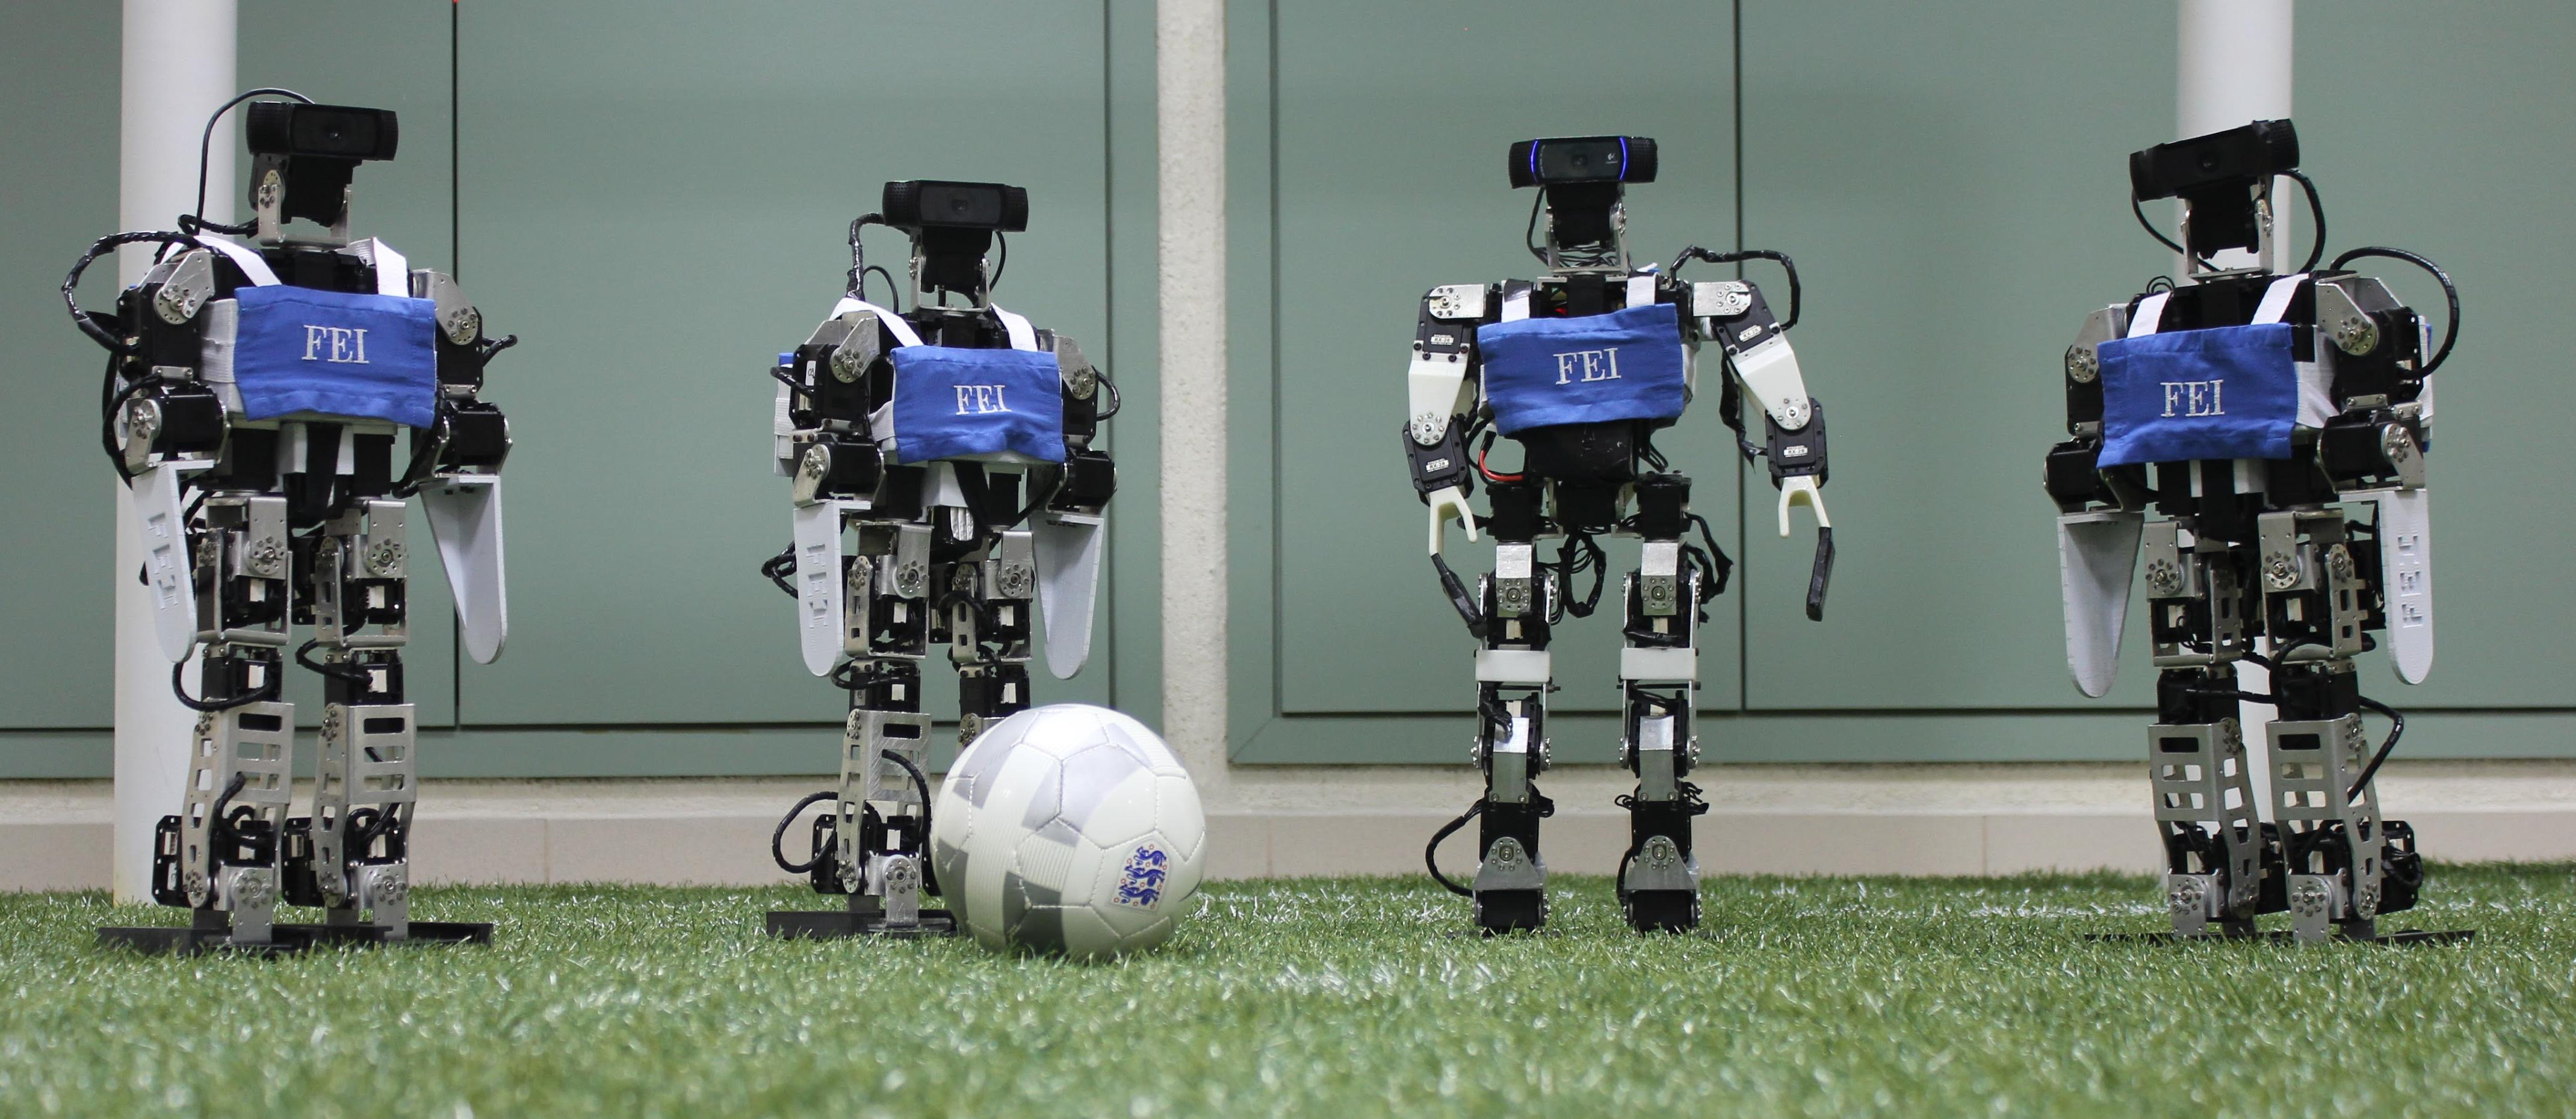
\includegraphics[width=\textwidth]{fig/team-2016}
\end{figure}

  \item \textbf{RoboFEI:} durante o período de mestrado, o autor participou ativamente do grupo de robótica da FEI, mais precisamente no time de futebol de robôs humanoides.
  Entre outras tarefas, o autor tinha o objetivo de desenvolver o sistema de localização que seria utilizado pelos robôs em jogo, além de participar dos eventos que envolviam a equipe.
  %
  O autor participou da Competição Latino-Americana de Robótica (LARC) de 2016, que foi realizada em Recife nos dias 10, 11 e 12 de Outubro de 2016.
  Nesta edição o autor junto com o time foram campeões da competição latino-americana de futebol de robôs humanoides, além de participar da competição da corrida de robôs humanoides.
  No período compreendendo do dia 27 à 30 de Julho de 2017 o autor participou da competição mundial RoboCup, que foi sediada em Nagoya no Japão.
  Além destas, a equipe também participou da RoboCup que ocorreu em Leipzig na Alemanha entre os dias 30 de Junho e 3 de Julho de 2016.

  \item \textbf{Aulas Voluntárias:} durante o período em que o autor fez parte do programa de mestrado da FEI, ele foi professor de um curso de férias do dia 6 ao dia 10 de Fevereiro de 2017, onde foram apresentados conceitos fundamentais das linguagens de programação C++ e Python para alunos da graduação da FEI.
  Além delas, foram ministradas aulas semanais de laboratório para uma turma de graduação de Maio à Junho de 2017, onde foram ministradas 6 aulas.

  \item \textbf{Outros Eventos:} além dos eventos citados, houveram as participações no FEI Portas Abertas, nas edições de 2016 e 2017, que é um evento onde alunos de ensino médio são convidados à conhecer as dependências e os projetos desenvolvidos pela FEI.
  Também houve a participação na Feira do Guia do Estudante de 2016.

\end{enumerate}

Assim, foram apresentadas as atividades desenvolvidas pelo aluno durante o período vigente da bolsa concedida pelo CNPq.

%--------------------------------------------------------------------------------------------------

\chapter{Resultados Obtidos}

Além de uma implementação completa do sistema de localização para robôs humanoides autônomos, as contribuições deste trabalho para o estado da arte do método de localização de Monte-Carlo são: a utilização dos pesos das partículas como fator para dispersar partículas com baixa representatividade, a utilização do desvio padrão das posições das partículas para determinar a quantidade de partículas necessárias para representar a distribuição de probabilidades e o método que estima qual observação deve fornecer a informação que melhora o desempenho do sistema de localização.
Todas essas contribuições apresentadas foram tema da dissertação de mestrado apresentada para a obtenção do título de mestre pelo autor.

Além da dissertação, como resultado dos trabalhos citados nos capítulos anteriores foi feita uma tentativa de publicação, para o Simpósio Latino-Americano de Robótica (LARS) de 2016, o artigo foi rejeitado.
No entanto, um artigo em co-autoria com outros integrantes do grupo de robótica foi aceito, e o autor fez uma apresentação em inglês sobre o artigo durante o simpósio que ocorreu em 13 de Outubro de 2016.
O artigo de \citeonline{perico2016robot} apresenta o simulador que foi desenvolvido pela equipe com o objetivo de auxiliar no desenvolvimento de algoritmos de inteligência artificial.

Em 2017, o autor escreveu um artigo que foi aceito para publicação para a edição do LARS de 2017.
Neste artigo \citeonline{almeida2017vision} apresentam alguns trechos da pesquisa desenvolvida para a dissertação de mestrado do autor.

O autor recebeu o prêmio de melhor time da liga humanoide de futebol de robôs do campeonato Latino-Americano (LARC) de 2016, conforme o que já foi apresentado no capítulo anterior.

%--------------------------------------------------------------------------------------------------

\chapter{Considerações Finais}

Finalmente, após esses dois anos, em que o autor teve a oportunidade de se desenvolver academicamente os resultados foram:
%
\begin{enumerate}
  \item um artigo publicado como co-autor;

  \item um artigo publicado como autor;

  \item uma apresentação feita em um simpósio internacional;

  \item participações em duas competições internacionais;

  \item participações em diversos eventos de fomento à robótica no país;

  \item e a obtenção do título de mestre.
\end{enumerate}

A dedicação em período integral ao mestrado só foi possível devido à bolsa auxílio fornecida pelo CNPq.
E sem essa dedicação integral seria praticamente impossível gerar publicações ou até mesmo participar mais ativamente do desenvolvimento da área no país.

% ----------------------------------------------------------
% Introdução (exemplo de capítulo sem numeração, mas presente no Sumário)
% ----------------------------------------------------------

\postextual

% ----------------------------------------------------------
% Referências bibliográficas
% ----------------------------------------------------------
\bibliography{bib}
\end{document}